
\section{Current and Future Work: Deep Latent Variable Modeling}

\begin{frame}
\begin{center}
    \textbf{Research Direction: Deep Latent-Variable Models for NLP }
  \end{center}
  Goal: Expose specific choices as explicit latent variables.   
  
\end{frame}

\begin{frame}
\begin{center}
    \textbf{ Latent-Variable Model Basics }
  \end{center}
  
Latent variable models give us a joint distribution
\begin{align*}
p(x, z \param \theta).
\end{align*}

\pause
\begin{itemize}
    \item $x$ is our observed data
    \item $z$ is a collection of latent variables
    \item $\theta$ are the deterministic parameters of the model, such as the neural network parameters
\end{itemize}

\pause

\begin{itemize}
    \item Data consists of $N$ i.i.d samples,
\end{itemize}


                \[ p(x^{(1:N)}, z^{(1:N)} \param \theta ) = \prod_{n=1}^N p(x^{(n)} \given z^{(n)}; \theta) p(z^{(n)};\theta). \]
\end{frame}

\begin{frame}\thetitle{Posterior Inference}
    For models $p(x, z \param \theta)$, we'll be interested in the \textit{posterior} over latent variables $z$:
    
    \begin{align*}
        p(z \given x \param \theta) = \frac{\displaystyle p(x, z \param \theta)}{\displaystyle p(x \param \theta)}.
    \end{align*}
    
    \air
    
    \air
    \pause
    Why?
    \begin{itemize}
        \item $z$ will often represent interesting information about our data (e.g., the cluster $x^{(n)}$ lives in, how similar $x^{(n)}$ and $x^{(n+1)}$ are).
        
        \item Learning the parameters $\theta$ of the model often requires calculating posteriors as a subroutine. \item Intuition: if I know likely $z^{(n)}$ for $x^{(n)}$, I can learn by maximizing $p(x^{(n)} \given z^{(n)} \param \theta)$.
        % \begin{itemize}
        %     \item Intuition: if I know likely $z^{(n)}$ for $x^{(n)}$, I can learn by maximizing $p(x^{(n)} \given z^{(n)} \param \theta)$.
        % \end{itemize}
    \end{itemize}
    
\end{frame}

\begin{frame}
  \begin{center}
    \textbf{ Example: Copy-Attention \\
      \small{(Gu et al, 2016) (Gulcehre et al, 2016)}}
  \end{center}

Let $z$ be a binary latent variable. 
\air
\begin{itemize}
\item If $z = 0$, let the model generate a new word. 
\item If $z = 1$, let the model copy a word from the source.   
\end{itemize}

Inference:

\begin{center}
  

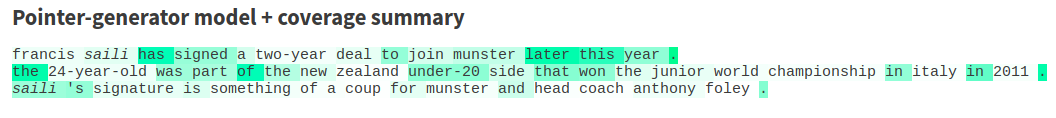
\includegraphics[width=15cm]{seeblog}

\centerline{\small (See et al, 2017)}
\end{center}
\end{frame}


\begin{frame}
  \begin{center}
    \textbf{ Latent Variable Models for Generation}
  \end{center}
  
  \begin{itemize}
  \item Can we develop other discrete latent-variable models for generation?
    \air
  \item Perhaps each important aspect of generation can be built-in directly.
    \air
  \item Goals:
    \begin{itemize}
    \item Model Control 
    \item Model Debugging
    \item Model Uncertainty
    \end{itemize}
  \end{itemize}
\end{frame}



\begin{frame}
  \begin{center}
    \textbf{Approach 1: Latent Alignment and Variational Attention}
  \end{center}
  
  \begin{center}
    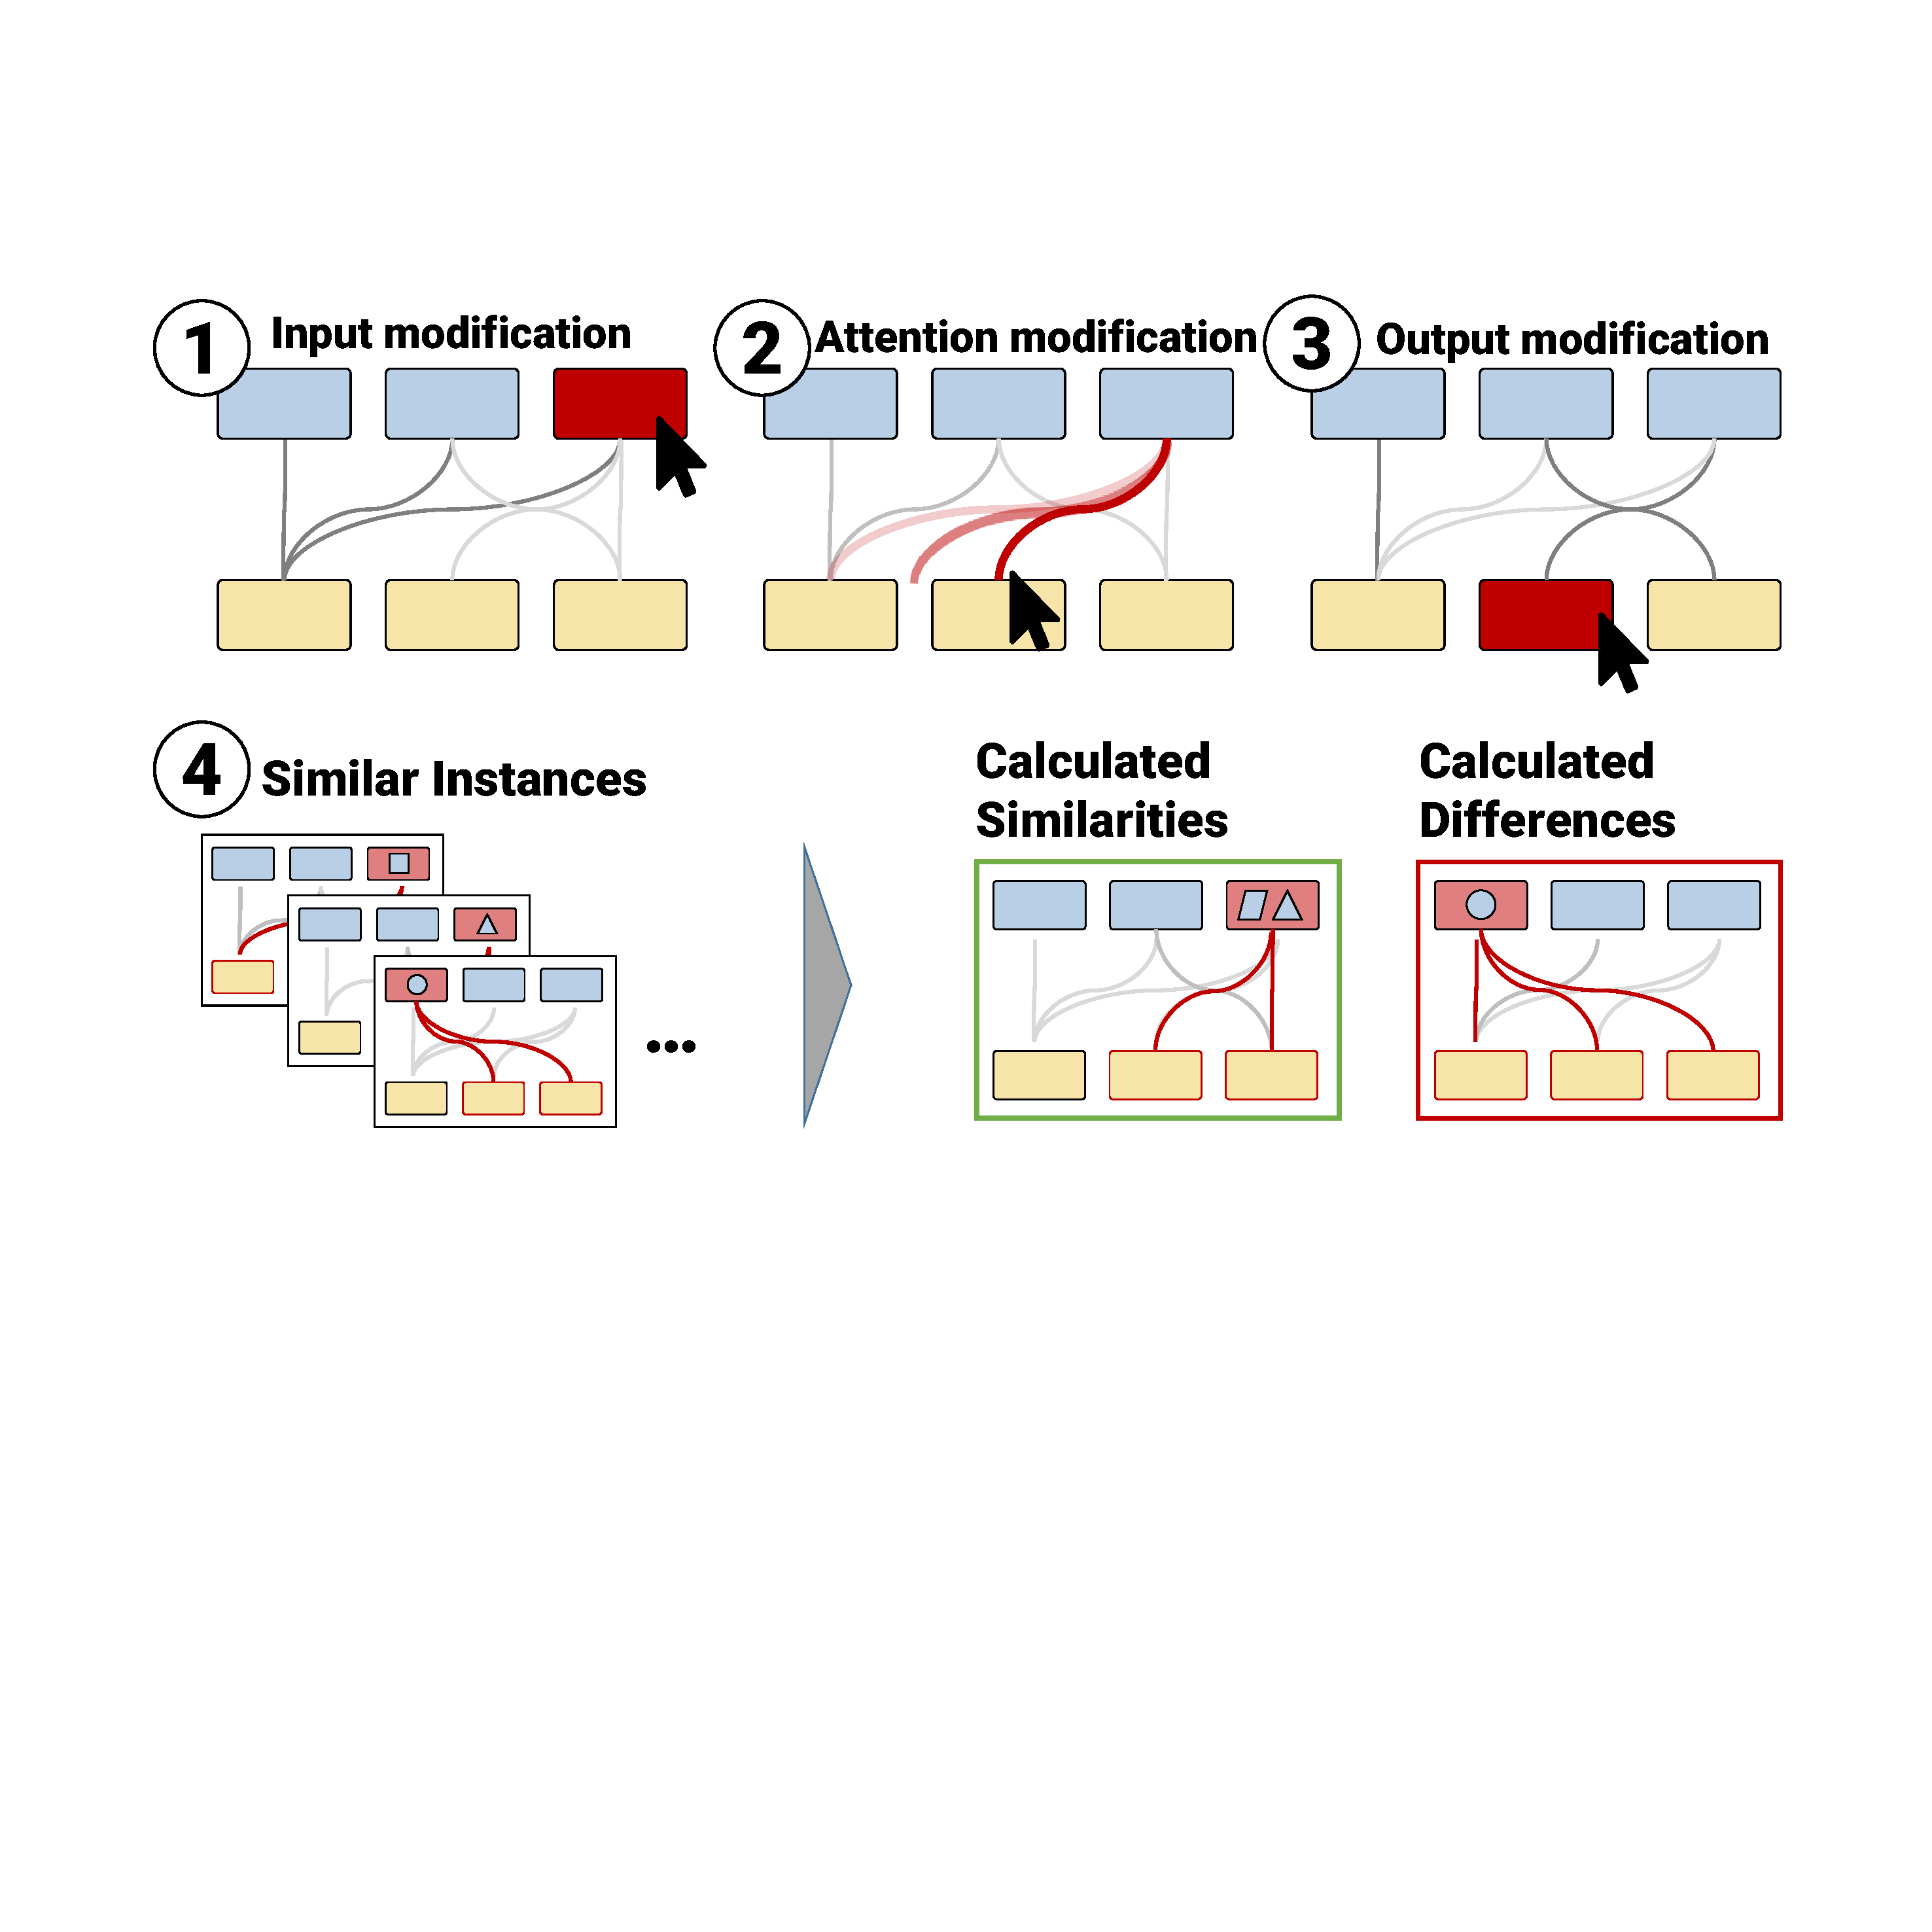
\includegraphics[width=0.7\textwidth]{AttentionVIS}
  \end{center}
\end{frame}


\begin{frame}
  \begin{center}
    \textbf{Approach 2: Learning Neural Templates}
  \end{center}

  \begin{center}
    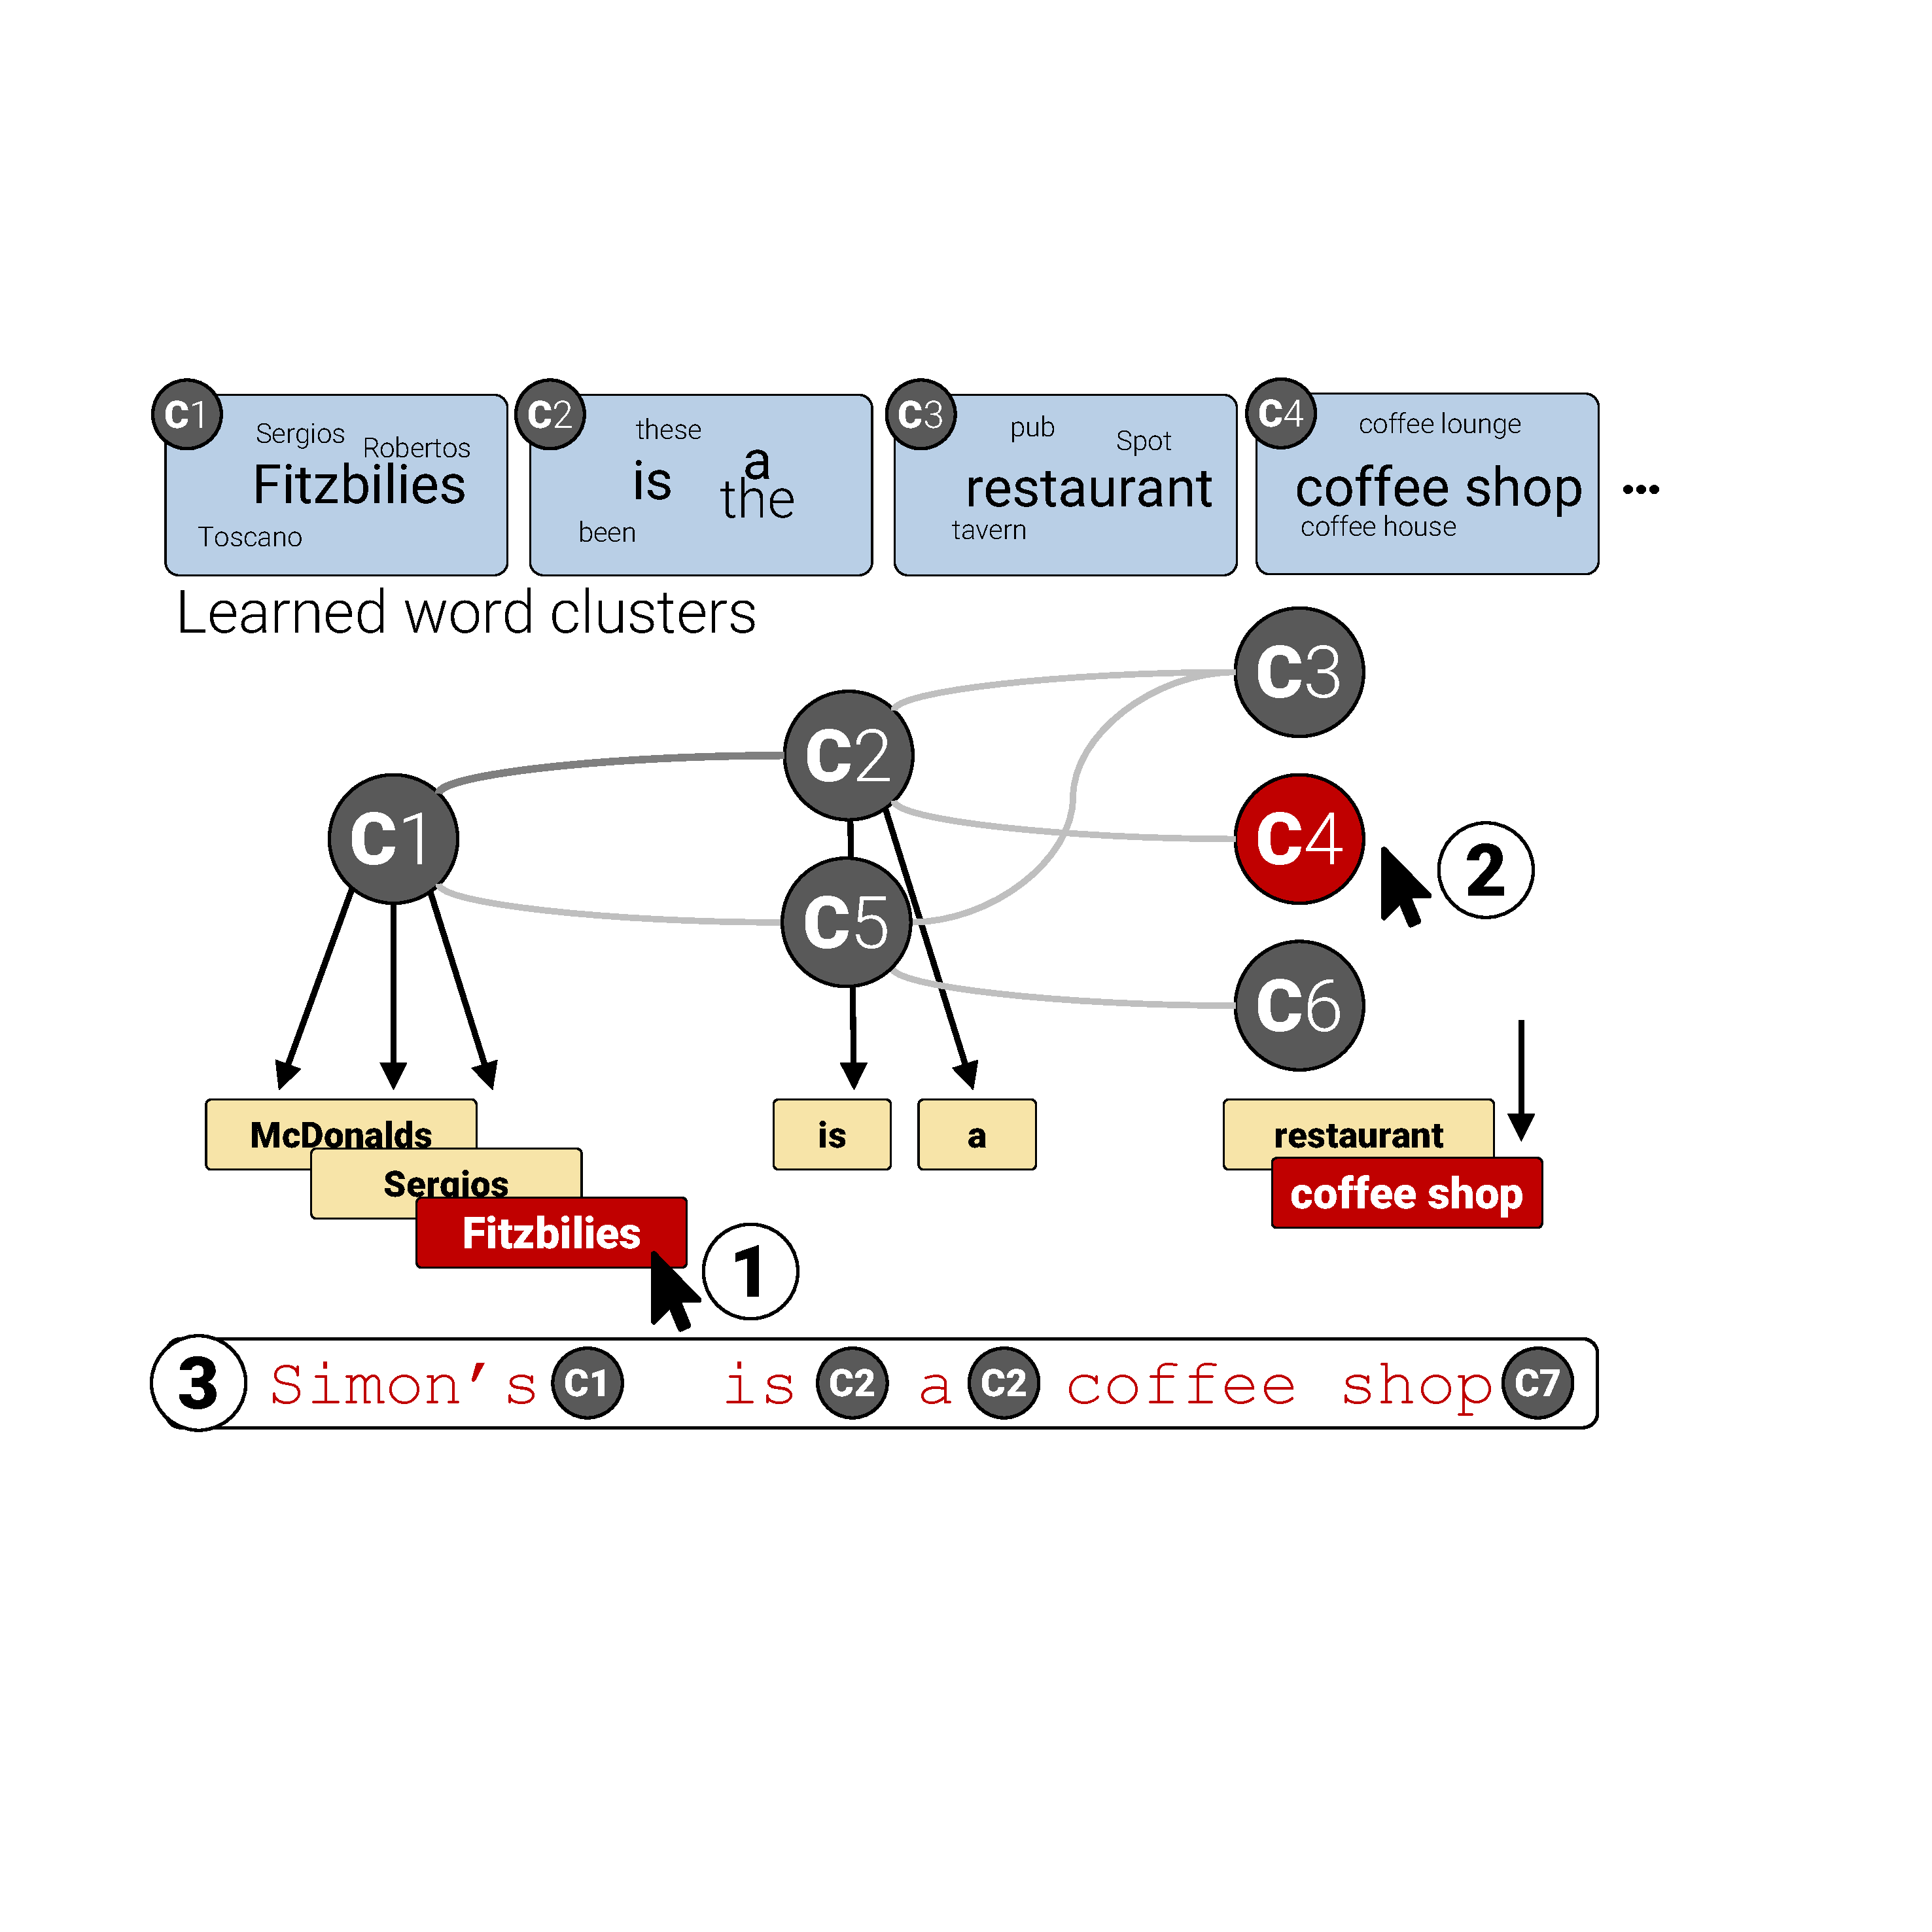
\includegraphics[width=0.7\textwidth]{DecoderVis}
  \end{center}
\end{frame}


\begin{frame}{}

\end{frame}

\begin{frame}

\end{frame}

\section{Impact and Outreach}

\begin{frame}{OpenNMT}

\end{frame}

\begin{frame}{LSTMVis}

\end{frame}



\section{Future Work}

\begin{frame}{Probabilistic Programming}

\end{frame}

\begin{frame}{Probabilistic Programming}

\end{frame}


\begin{frame}

\end{frame}
